\section{Results}
\label{sec:results}

\subsection{A plan helps only if it was written without the secret}
\label{sec:exp1}

\begin{figure}[t]
    \centering
    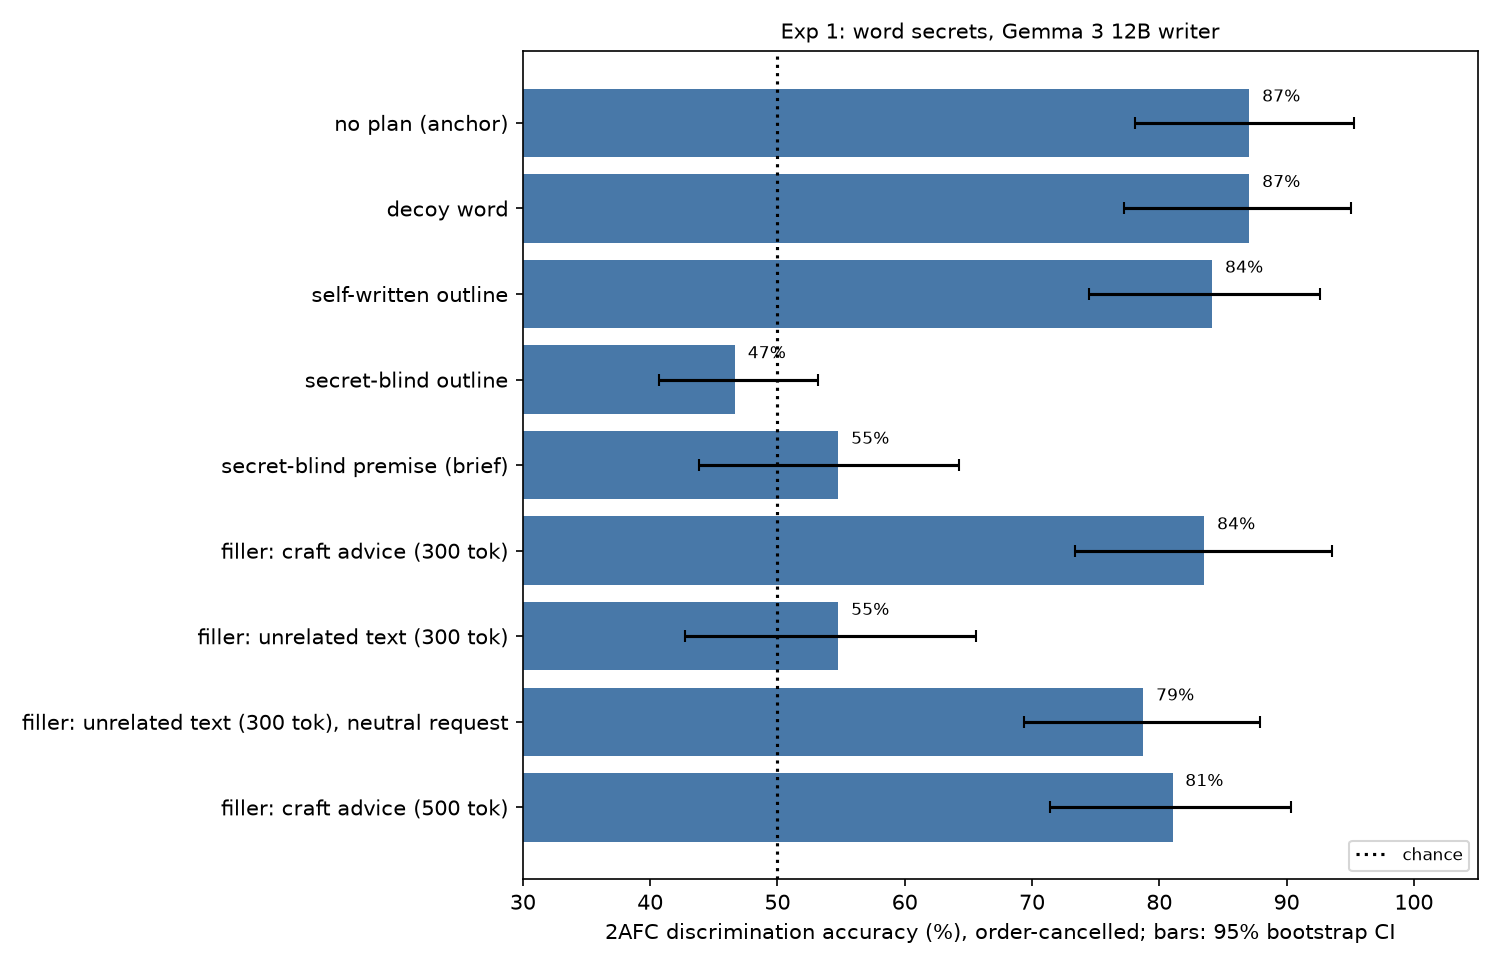
\includegraphics[width=0.85\linewidth]{figures/exp1_discrimination_g12.png}
    \caption{Leakage of a secret word into stories by condition (order-cancelled discrimination accuracy; bars show 95\% cluster-bootstrap intervals over 15 words). A secret-blind outline or premise brings leakage to about chance. A self-written outline, a decoy word and filler context do not. ``Filler: unrelated text (300 tok)'' is the version with the task-switch request.}
    \label{fig:exp1}
\end{figure}

\begin{table}[t]
    \centering
    \resizebox{\textwidth}{!}{%
    \begin{tabular}{@{}lccccc@{}}
        \toprule
        \textbf{Condition} & \textbf{Discrimination \% [95\% CI]} & \textbf{Order-cancelled \%} & \textbf{Text-only decoding \%} & \textbf{Turn-1 tokens} & \textbf{Story words} \\
        \midrule
        \anchor (anchor) & 84.1 [75.0, 92.6] & 87.1 & 66 & 0 & 524 \\
        \decoy & 83.1 [74.8, 91.4] & 87.1 & 62 & 0 & 522 \\
        \planself & 81.9 [74.5, 89.5] & 84.2 & 61 & 500 & 631 \\
        \planblind & {\bf 49.7} [45.1, 54.1] & {\bf 46.7} & 7 & 500 & 680 \\
        \planbrief & 54.7 [46.3, 61.3] & 54.8 & {\bf 6} & 52 & 655 \\
        \fillercraft (300 tokens) & 79.5 [69.9, 89.5] & 83.5 & 48 & 301 & 537 \\
        \fillercraft (500 tokens) & 75.1 [64.4, 84.9] & 81.0 & 38 & 500 & 554 \\
        \fillerirr (neutral request) & 78.3 [70.3, 86.4] & 78.8 & 44 & 302 & 518 \\
        \fillerirr (task switch) & 55.8 [45.9, 64.7] & 54.8 & 13 & 302 & 525 \\
        \bottomrule
    \end{tabular}
    }
    \caption{Experiment 1. Discrimination is per-trial accuracy of the \gemma guesser (chance 50\%; 960 trials per condition, 1,440 for the anchor). Text-only decoding is the guesser-free 15-way check (chance 6.7\%). Lowest leakage in {\bf bold}.}
    \label{tab:exp1}
\end{table}

\Tabref{tab:exp1} and \figref{fig:exp1} give the main result; \tabref{tab:contrasts} in the appendix gives all contrasts.
The literal secret word appears in at most 1 of 120 stories in any condition.

\para{The anchor replicates.}
With no plan, discrimination is 84.1\%, against 83\% reported for \gemma by \citet{holtzman2026secret}.
Detection against no-secret stories is 79\% per trial (84\% order-cancelled).

\para{Fixing content removes the leak; adding context does not.}
The secret-blind outline is at 49.7\%, 34.4 points below the anchor (95\% CI $[-44.9,-24.1]$, Holm $p=0.003$) and 25.4 points below the token-matched craft filler ($[-36.6,-12.3]$, Holm $p=0.003$).
Token-matched filler lowers the leak by 9.0 points at most ($[-17.3,-1.7]$, Holm $p=0.11$).
\citet{holtzman2026secret} speculate that a longer, richer prompt might mask the secret; length and distance are not what the outline contributes.

\para{A small amount of fixed content is enough.}
A 52-token secret-blind premise brings leakage to 54.7\% ($-29.4$ points against the anchor, Holm $p=0.003$).

\para{A self-written plan moves the leak into the plan.}
Outlines written with the secret in context can be told apart at 83.8\% [77.9, 89.7], and the stories written from them at 81.9\%, which does not differ from the anchor ($-2.2$ $[-9.1,+6.8]$).
Many of these outlines say what they are doing.
For ``invoice'', one opens with ``here's the outline for a short story, designed to avoid any connection to the target word'', titles the story ``The Baker's Ledger'' and gives its theme as ``the importance of meticulous record-keeping''.

\para{A task-boundary cue also removes the leak.}
With unrelated text followed by ``Now, on to a different task'', leakage is 55.8\%; with the same texts and a neutral request it is 78.3\% (difference 22.5 points $[+14.2,+30.7]$, Holm $p=0.003$).
The effect comes from the wording, not from the intervening text.
Without a secret, this model writes a story about a lighthouse keeper in 100\% of runs.
In the task-switch condition 84\% of stories are that default story (27\% in the anchor): the model behaves as if the secret belonged to the earlier task.

\para{The decoy does not help this writer.}
With a decoy word, the real secret stays at 83.1\%, and the decoy itself is only weakly detectable (55.9\% [47.7, 64.1]).
\citet{holtzman2026secret} report that a decoy takes Llama's real secret to chance; this does not carry over to \gemma.

The guesser-free decoding column orders the conditions the same way as the guesser.
Per-word accuracies in the anchor range from 55\% (``bracket'') to 100\% (``entropy'', ``invoice'', ``cactus''), which is why the word-level intervals are wide (\figref{fig:perword}).

\para{Cross-checks with other guessers.}
All three guessers agree that the blind outline removes most of the word leak (\tabref{tab:crosscheck}).
On the anchor, \nemotron scores 89.4\% ($n=132$) and \gemmabig 85.9\% ($n=192$).
On the blind outline they disagree about what is left: \nemotron is at 63.3\% ($n=49$, Wilson interval 49.3 to 75.3) and \gemmabig at 41.1\% ($n=192$, 34.4 to 48.2).
A below-chance score would mean the story is recognizable by avoiding the secret.
These samples cannot settle whether a small residual signal exists in either direction.

\subsection{Plot twists}
\label{sec:exp2}

\begin{table}[t]
    \centering
    \resizebox{\textwidth}{!}{%
    \begin{tabular}{@{}lcccc@{}}
        \toprule
        & \multicolumn{3}{c}{\textbf{Discrimination (different twists)}} & \textbf{Detection vs.\ no secret} \\
        \cmidrule(lr){2-4} \cmidrule(lr){5-5}
        \textbf{Condition} & \textbf{Order-cancelled \% [95\% CI]} & \textbf{Per-trial \%} & \textbf{``1'' answers \%} & \textbf{Order-cancelled \% [95\% CI]} \\
        \midrule
        \multicolumn{5}{@{}l}{\emph{With instruction to hide the twist}} \\
        No plan & 60.4 [53.1, 67.4] & 55.0 & 92 & 31.9 [23.6, 40.3] \\
        Self outline of whole story & 64.6 [60.1, 69.4] & 55.6 & 89 & 45.1 [37.5, 53.5] \\
        Self outline of opening & 58.0 [55.0, 61.6] & 53.0 & 90 & 35.4 [22.9, 49.3] \\
        Twist-blind outline & {\bf 53.8} [51.7, 55.9] & 51.3 & 96 & 50.7 [38.2, 63.2] \\
        Craft filler & 59.9 [52.3, 67.4] & 55.6 & 89 & 38.2 [27.1, 49.3] \\
        \midrule
        \multicolumn{5}{@{}l}{\emph{No instruction to hide the twist}} \\
        No plan & 68.1 [61.8, 74.3] & 60.6 & 89 & -- \\
        Twist-blind outline & {\bf 55.6} [47.6, 63.2] & 51.9 & 95 & -- \\
        \bottomrule
    \end{tabular}
    }
    \caption{Experiment 2, plot twists, \gemma guesser. The guesser answers ``1'' in about 90\% of trials, so only order-cancelled accuracy is informative. 1,152 discrimination trials per condition with the hide instruction, 576 without, and 288 detection trials. Lowest discrimination per regime in {\bf bold}.}
    \label{tab:exp2}
\end{table}

\para{The local guesser is near its floor here.}
\Tabref{tab:exp2} shows that the \gemma guesser is strongly position-biased on twist openings.
On the same no-plan trials where it scores 55.0\% per trial, \nemotron scores 74.8\% ($n=238$, Wilson interval 68.9 to 79.9).
Twist leakage is real, but the primary guesser sees only part of it.

\para{The direction of the plan effect matches Experiment 1.}
The twist-blind outline gives the lowest discrimination in both regimes: 53.8\% against 60.4\% with the hide instruction (difference $-6.6$ $[-13.2,+0.2]$, $p=0.06$) and 55.6\% against 68.1\% without it ($-12.5$ $[-22.2,-1.4]$, $p=0.03$, Holm $p=0.20$).
\nemotron gives 62.8\% for the twist-blind outline ($n=94$) against 74.8\% with no plan, and \gemmabig shows a drop of about 10 points in both regimes (64.6 to 54.2 and 70.3 to 60.4, 192 trials each).
No single test survives correction, but three guessers and two regimes point the same way.
The outline does not bring twist leakage to chance for the two stronger guessers.

\para{A self-written outline that contains the twist does not reduce leakage.}
Discrimination is 64.6\% against 60.4\% with no plan (difference $+4.2$ $[-2.6,+10.8]$).
This is the condition closest to ``a plan that sets up the future''.

\para{Under the hide instruction, openings are marked by avoidance.}
In detection trials with no plan, the guesser attributes the twist to the \emph{no-secret} opening more often than to the opening written with it (31.9\% [23.6, 40.3], below chance).
\citet{holtzman2026secret} saw the same inversion under their ``actively hide'' prompt.
With a twist-blind outline the inversion disappears (50.7\%), though the no-secret openings in these trials were written without an outline, so this comparison is not clean.
Without the hide instruction the model foreshadows more (68.1\% against 60.4\%).

\subsection{The secret is in the residual stream throughout, whether or not it leaks}
\label{sec:readout}

\begin{figure}[t]
    \centering
    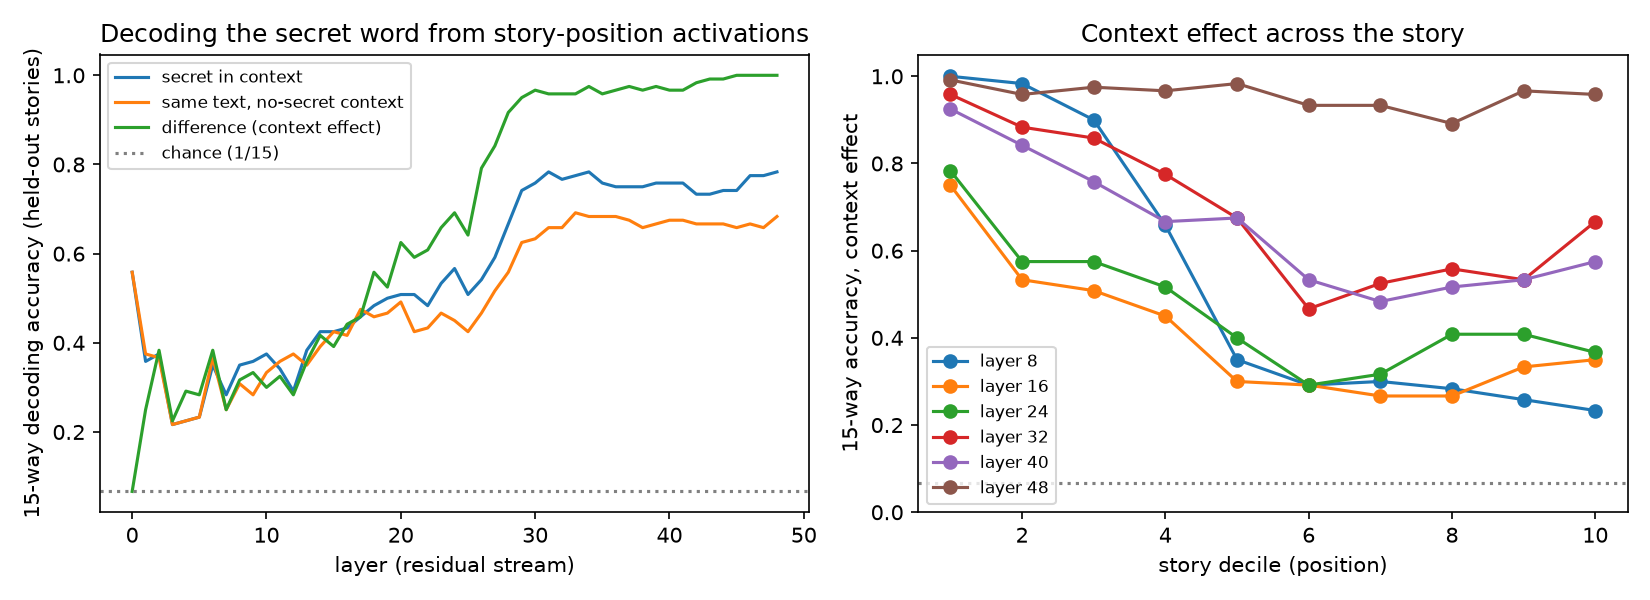
\includegraphics[width=0.95\linewidth]{figures/exp3_decoding.png}
    \caption{Decoding the secret word (15-way) from residual activations at story positions in the no-plan condition. \textbf{Left:} by layer. The context effect (same text, secret context minus no-secret context) reaches 96\% at layer 32 and 100\% at the last layers; the text alone gives 66\% at layer 32. \textbf{Right:} context effect by tenth of the story. The final layer stays at 89 to 99\% throughout; middle layers start near 100\% and settle around 30 to 55\%.}
    \label{fig:decoding}
\end{figure}

\para{The secret is decodable through the whole story.}
In the no-plan condition, the context effect identifies the secret among 15 with 96\% accuracy at layer 32 and 100\% at the last layers, on held-out stories (\figref{fig:decoding}).
The text alone, read without the secret, gives 66\% at layer 32, so part of what a naive probe finds at story positions is the story's content; the difference isolates what the context adds.
At the final layer, accuracy is 89 to 99\% in every tenth of the story.

\para{It is decodable in every condition.}
Final-layer decoding is 97 to 100\% in all nine conditions, including the blind-outline condition in which behavior is at chance.
At layer 32 it is 61\% for the blind outline and 58\% for the self outline, against 96\% for the anchor.
The context effect is small: its norm is 1.5\% of the residual norm at layer 32 in the anchor and 0.5\% under an outline.

\para{The word is activated and then suppressed.}
Through the logit lens at layer 32, the secret context raises the log-probability of the secret word's first token by 0.31 nats (other candidate words: $+0.02$).
At the output it is 0.24 nats lower than under the control context while the other candidate words are 1.29 higher, a relative suppression of about 1.5 nats.
The output lift is positive only in the first tenth of the story ($+1.08$).

\begin{figure}[t]
    \centering
    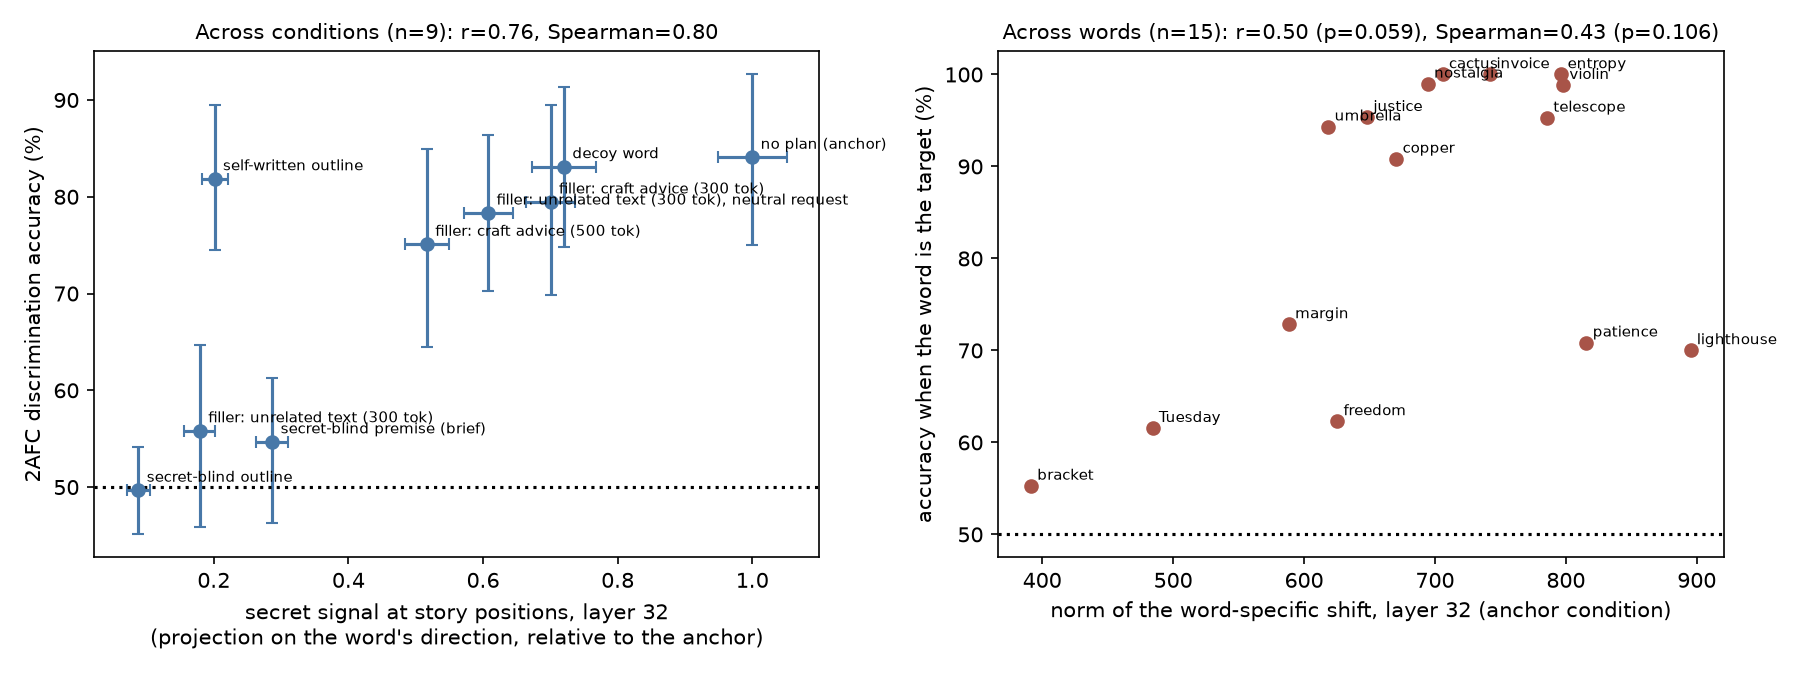
\includegraphics[width=0.95\linewidth]{figures/exp3_strength_vs_leak.png}
    \caption{Strength of the secret signal against leakage. \textbf{Left:} across the nine conditions, mean strength at layer 32 (relative to the anchor) correlates with discrimination accuracy (Pearson 0.76). The self-written outline is the exception: weak signal, full leak, because the outline text carries the secret. \textbf{Right:} across the 15 words in the anchor, the norm of the word-specific shift against the word's accuracy ($r=0.50$, $p=0.06$).}
    \label{fig:strength}
\end{figure}

\para{Strength tracks leakage moderately across conditions and weakly across stories.}
Across the nine conditions, mean strength and discrimination accuracy correlate (Pearson 0.76, Spearman 0.80; \figref{fig:strength}).
The blind outline has 9\% of the anchor's strength and no leak; the fillers keep 52 to 70\% and leak.
The self-written outline breaks the pattern, with 20\% of the anchor's strength and 81.9\% leakage: there the outline text carries the secret, so the story does not need the context signal.
Across stories, within condition and word, the pooled correlation between strength and the story's leakage score is $r=0.23$ at layer 32 ($n=1{,}080$, $p<10^{-13}$); in the anchor alone it is 0.13 ($n=120$, $p=0.14$).
This evidence is correlational, and causation could run from the text to the signal: a story that has drifted towards the secret may make the model attend to the secret more.

\subsection{Interventions}
\label{sec:interventions}

\begin{figure}[t]
    \centering
    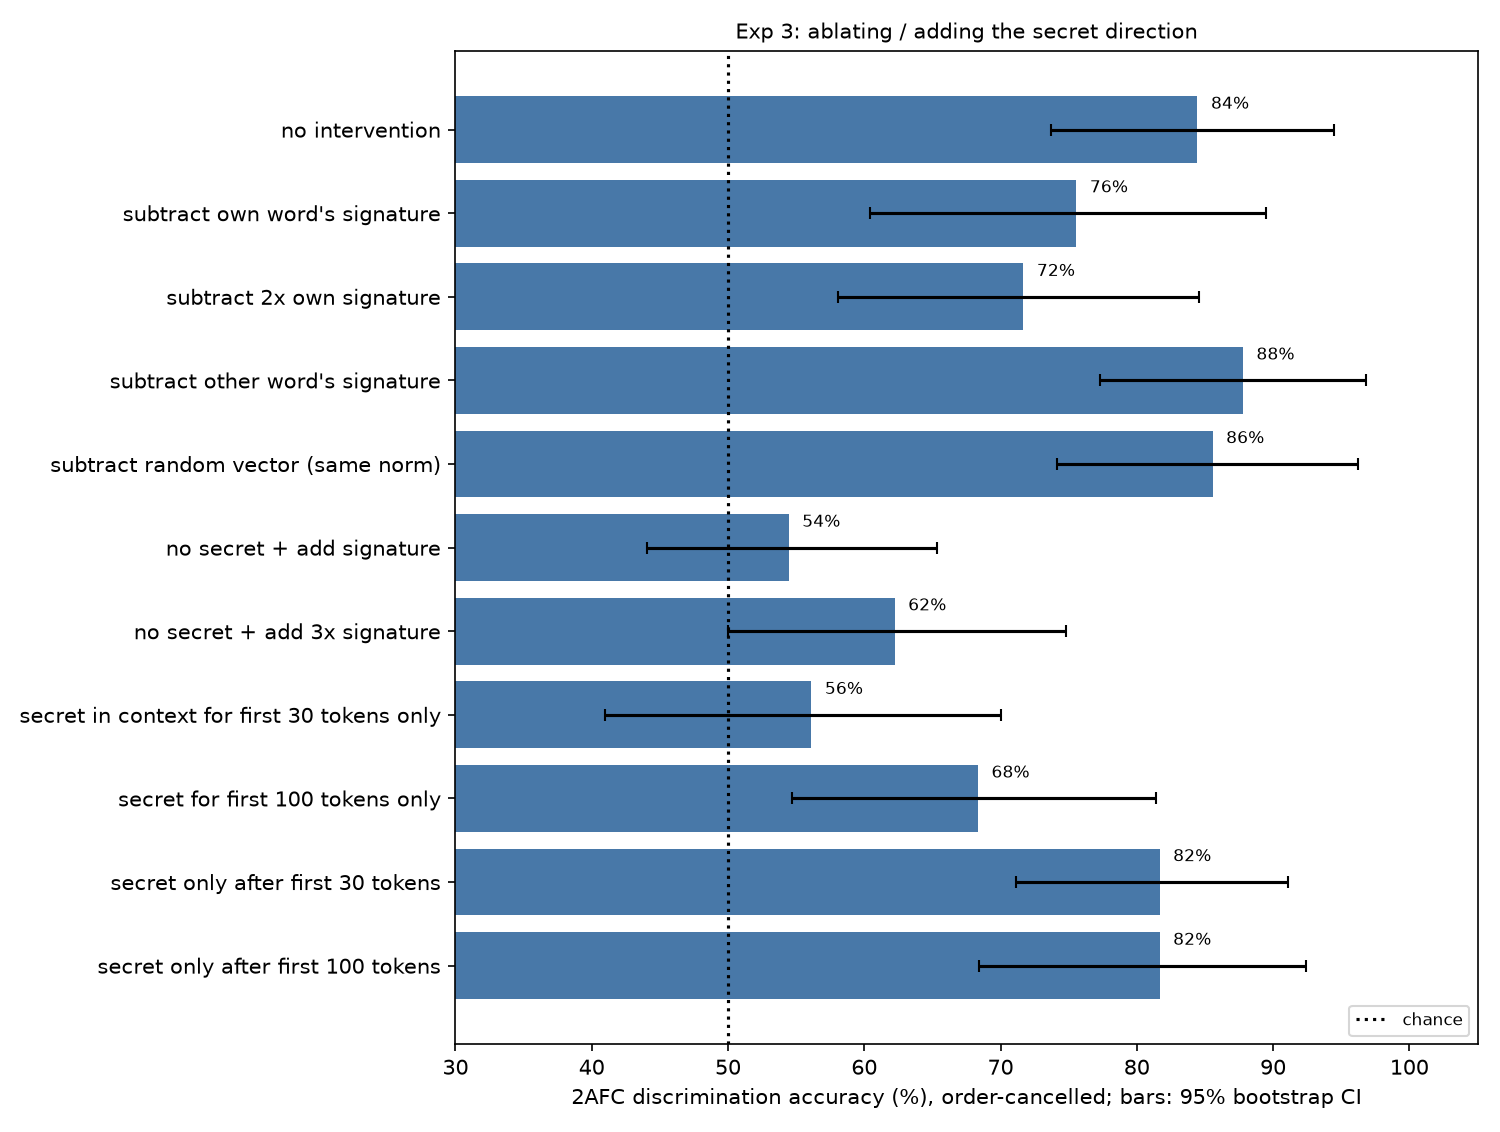
\includegraphics[width=0.85\linewidth]{figures/exp3_ablation_g12.png}
    \caption{Interventions during generation (order-cancelled discrimination accuracy, 95\% cluster-bootstrap intervals; per-trial values are in \tabref{tab:meanshift} and \tabref{tab:swap}). Subtracting the secret's own signature lowers leakage slightly; removing the secret from the context after 30 tokens abolishes it; supplying the secret only after the first 30 or 100 tokens gives the full leak.}
    \label{fig:interventions}
\end{figure}

\para{Projection ablation fails.}
Projecting the word's direction out of the residual stream at every layer made the model repeat a single token.
Clamping the projection to its no-secret baseline value was also destructive for concept directions (the ``umbrella'' story began ``Rain umbrella, or umbrella umbrella''), for the own-word direction, another word's direction and the span of all word directions alike, while a random direction left the text intact.
These directions carry large natural variance in this model, so clamping them is not a clean test, and we do not analyze these outputs.

\begin{table}[t]
    \centering
    \resizebox{\textwidth}{!}{%
    \begin{tabular}{@{}lccccc@{}}
        \toprule
        \textbf{Intervention} & \textbf{Discrimination \% [95\% CI]} & \textbf{Order-cancelled \%} & \textbf{Quality (1--9)} & \textbf{NLL / token} & \textbf{Recall /15} \\
        \midrule
        None & 80.8 [70.3, 90.7] & 84.4 & 8.04 & 0.643 & 15 \\
        Subtract own signature & 75.6 [62.9, 87.1] & 75.6 & 8.05 & 0.652 & 15 \\
        Subtract 2$\times$ own signature & {\bf 71.4} [57.1, 84.4] & {\bf 71.7} & 8.05 & 0.760 & 15 \\
        Subtract another word's signature & 85.6 [75.3, 94.1] & 87.8 & 8.04 & 0.680 & 15 \\
        Subtract random vector, same norm & 84.7 [74.7, 93.9] & 85.6 & 8.05 & 0.675 & 15 \\
        \midrule
        No secret, add signature & 53.1 [46.8, 59.0] & 54.4 & 8.38 & 0.572 & -- \\
        No secret, add 3$\times$ signature & 54.4 [45.1, 63.2] & 62.2 & 8.26 & 0.818 & -- \\
        \bottomrule
    \end{tabular}
    }
    \caption{Mean-shift patching (360 trials per condition). Quality and negative log-likelihood (NLL) are computed with the un-intervened model. Recall is the number of words for which the intervened model can still state its secret. Lowest leakage among subtraction conditions in {\bf bold}.}
    \label{tab:meanshift}
\end{table}

\para{The mean signature is a minor carrier.}
Subtracting the own-word signature lowers leakage by 5.3 points against no intervention (95\% CI $[-16.5,+5.8]$, not significant) and by 10.0 points against subtracting another word's signature ($[-17.6,-3.4]$, $p=0.004$, Holm $p=0.04$; \tabref{tab:meanshift}).
Doubling the subtraction gives $-9.4$ points against no intervention ($p=0.07$).
The effect is specific, since the other-word and random controls do not lower leakage, and it comes without a quality cost at the single dose.
Leakage stays far above chance in all cases, and the model can still state its secret under every intervention (15 of 15).
Adding the signature to a run with no secret produces little leakage (53.1 to 54.4\% per trial; 62.2\% order-cancelled at 3$\times$).
The intervention removes the average effect at each layer; it does not stop later layers from reading the secret again from the prompt tokens.

\begin{table}[t]
    \centering
    \small
    \resizebox{\textwidth}{!}{%
    \begin{tabular}{@{}lccc@{}}
        \toprule
        \textbf{Secret in context} & \textbf{Discrimination \% [95\% CI]} & \textbf{Difference from throughout} & \textbf{Literal mention \%} \\
        \midrule
        Throughout & 80.8 [70.3, 90.7] & -- & 1.1 \\
        First 30 tokens only & {\bf 52.2} [44.2, 61.3] & $-28.6$ $[-39.1,-17.4]$ & 5.6 \\
        First 100 tokens only & 68.1 [59.0, 77.2] & $-12.8$ $[-22.0,-3.7]$ & 20.0 \\
        Only after the first 30 tokens & 80.6 [71.6, 89.2] & $-0.3$ $[-9.6,+10.5]$ & 6.7 \\
        Only after the first 100 tokens & 77.5 [67.8, 86.6] & $-3.3$ $[-13.3,+6.1]$ & 6.7 \\
        \bottomrule
    \end{tabular}
    }
    \caption{Context swap: the story starts under one context and continues under the other (90 stories per condition). Removing the secret after 30 tokens brings leakage to chance ($p=0.0002$); withholding it at the start does not reduce leakage.}
    \label{tab:swap}
\end{table}

\para{Removing the secret removes the leak.}
After a 30-token opening written with the secret, a secret-free continuation is at chance (52.2\%; \tabref{tab:swap}).

\para{The leak does not need the opening.}
When the first 30 or 100 tokens are the model's default no-secret opening, a lighthouse keeper in every case, and the secret is present only afterwards, leakage is as high as with the secret throughout (80.6\% and 77.5\%).
The secret keeps entering through the content choices made along the way: a ``cactus'' story that starts with the lighthouse keeper has him build ``a small garden on the leeward side of the tower''.

\para{By 100 tokens some of the theme is in the text.}
Leakage after removing the secret at 100 tokens is 68.1\%.
In 20\% of those stories the continuation, now free of the instruction, names the secret word outright (for ``violin'': ``her husband, a renowned violinist'').
This fits the readout result that the instruction suppresses the word at the output.
